\documentclass[12pt]{article}
\usepackage{amsmath, amsthm, amssymb, pdfpages} 
\usepackage{fullpage}
\usepackage{hyperref}
\usepackage{graphicx}
\usepackage[capitalize]{cleveref}


\title{Test the Effectiveness of Principal Components in Adjusting for Relatedness in Genetic Association Studies}

\author{Alex, Yiqi }





\usepackage{color}
\newcommand{\myred}[1]{{\color{red} #1}}



%%% To set proper spacing
\usepackage[vcentering,dvips]{geometry} 
\geometry{papersize={8.5in,11in},total={6.5in,8.5in}} 
\renewcommand{\baselinestretch}{1.15}
\begin{document}
	\maketitle
	
	
\section{Introduction} 

Genome-wide association study (GWAS) has been widely used to investigate whether target Single Nucleotide Polymorphism (SNP) is associated with certain trait (association study). However, considering admixture population is involved in recent study, failure to correct for population structure can reduce statistical power of GWAS. Hence, principal component analysis (PCA) which is a dimensionality-reduction method is used to provide examination for admixture population to identify the causal locus [2,3]. Although in recent study PCA has been a standard method to investigate the GWAS, doubts are cast on its statistical power and type one error controlling when comparing with other existing implementation such as linear mixed model (LMM) and Linear Regression (LM) [4]. Since current studies mainly focus on simple simulations or observation on real data [4, 5], existing evaluation can be limited to fully investigate the statistical power of PCA. In this paper, both simulation and real data set are used to evaluate the performance of PCA under different situations.\\

In this paper, we run the simulation of PCA in the scenario of large sample size, small sample size and complex family stucture with desirbale admixture simulatoin and trait simulation. In addition to this, we also test the performance of LMM and LM with the samle situation to PCA to make comparison. The performance of thess methods are measured by type one error and power. In the case of large sample size, we find out that PCA has well control in both type one error and power when the number of Principal Components (PC) reaches the ture rank of genotype matrix or subpoulation minus one. However, PCA will be punished in power when the sample size is small and the number of PCs are much larger than the ture rank of genotype matrix but it is still robust to type one error. With the existence of family structure, the performance of PCA is not so well in type one error controlling but in terms of power, it is similar to the performance of PCA without complex family strcuture. Compared with the performance of LM, it can be seen that if the number of PCs used in PCA is larger than true rank of genotype matrix, PCA has better performance than LM in both type one error and power. Seldom do previous research make comparison between PCA and LMM directly. In this paper, we test the performacne of LMM and PCA under the same situation. According to results of simulation
 
\section{Method} 
\subsection{Theory connecting to kinship}

\subsection{PCA GWAS  is Equivalent to linear regression with covariate}
The original model in our project has the same structure to linear regression. We assume that in this model, there are n individuals and m genetic marker. The formula can be written as: $$Y=\mu+X \vec{\beta}+\vec{\epsilon}$$. Here, Y is a n*1 vector which represents trait value for each individual and X is a n*m genotype matrix. In addition, $\vec{\beta}$ and $\vec{\epsilon}$ are a n*1 vectors representing the coefficient of genetics marker and residuals separately. Here $\epsilon$ follows a normal distribution $N(0,\sigma)$. This model sometimes fails beacause the number of genetic market is much larger than the number of indivudual. Then, we introduce PCA to make approximations\\

In a PCA linear regression model, we can write it in the form of $$y=\mu+ \vec{X_{j}} {\beta}_{j}+U_{1:i} \nu+\vec{\epsilon}$$

Here Y still repesents the numerical value of trait of different individual and $\mu$ is the intercept. Both of them are n*1 vector. Meanwhile, $\vec{X_{j}}$ is a n*1 vector of $j_{th}$ genetic marker and in this csae, $\beta$ is a scale regression coefficient. Then, $U_{1:i}$ is a n*i matrix which is the first i Principal Components and $\nu$ is a n*1 coefficient vector for $U_{1:i}$. In the end, $\epsilon$ represnets the residual which follows a normal distribution $N(0,\sigma)$ which is the same to previous model. Then, we need to test the significance of each gemetic marker. The null hypothesis is ${\beta}_{j}$ equals to 0 and the model in this case can be written as $y=\mu+U_{1:i} \nu+\vec{\epsilon}$ for $j_{th}$ market. The alternative hypothesis is ${\beta}_{j}$ does not equal to 0. Therefore, we will conduct the F test to investigate whether the reduced model can have the same statistical power. If the p-values is small, which indicates this market is associated with trait.\\

In our simulation, each individual will be test 100000 SNPs (Single Nucleotide Polymorphism) and each for each loci (in total 100000), we will conduct linear regression separately.  The genotype of each loci will be combined with eigenvector of principal components matrix which is composed of eigenvectors we used in PCA.Regarding the eigenvector of principal component, it is calculated by decomposing the kinship matrix.  

\subsection{Admixture Simulation}
The construction of admixture population is mainly based on admixture simulation of Alex (2016). The related code of admixture simulation has been uploaded to Github with a R package called "bnpsd".  Some parameters are changed in order to better simulate under different situation. According to Alex (2016), the number of independent loci is 30000, in this paper the number of independent locus is 10000. The default value of Alex (2016) is 3, whereas in this project, it can be variable. Considering the difference among number of sub-population, the sample size of $i_{th}$ sub-population will be set as the smaller integer of the ratio of total sample divided by number of sub-population.\\
Regarding the family structure, the generation will be set to be 20 to simulate admixture population with the existence of family structure. Considering the large calculation cost during the generation process of admixture population with family structure, this data set will be treated as real data set. It will be used repeatedly to test performance of PCA under different situations with random traits.



\subsection{Trait Simulation}
The construction of trait simulation is based on a R package called "simtrait". This package constructs the complex trait simulation with user-defined causal loci and the desirable heritability of the trait. It can be used in both simulated data set and real data set if the kinship matrix is estimated correctly. \\
In our simulation,the function of trait can be written as $$y=G+ \epsilon$$ 
, where G represents the effect of genotype and $\epsilon$ represents the noise. The noise follows a normal distribution with mean zero and variacne equals to one minus hertability rate times desired parametric variance factor of the trait which is 1 in default. To obtain the genotype effect, marginal allele frequency will be calculated first and then, SNP will be randomly selected as causal index with random SNP coefficients. Then  coefficients of causal index will be scaled and centered to estimate the genotype effect, thereby obtaining the numerical value of traits of each causal loci.The rank of genotype effect equals to the number of true subpopulation minus one as we take intercept into consideration as well.  


\subsection{Result Examination Method}
In this paper, precision-recall curves and uniformity p-value test will be used to test the performance of PCA under different scenarios. Both two methods will be illustrated by boxplot.
\subsubsection{Precision-Recall Curves}
Precision-recall curve is a plot whose y-axis represents precision and x-axis represents recall. Precision is calculated as the number of true positives divided by sum of both true positives which indicates the performance of model in predicting positives. Similarly, recall measures the ratio of number of true negatives and sum of true negatives and false negatives, which measures the performance of model in predicting negatives.Hence, the precision measures the relevancy of result which indicates the proportion of selected items are relevant. The recall shows the proportion of relevant items are selected. The precision and recall curve demonstrates the trade-off among precision and recall. Hence, the formula of precision and recall can be written as:
$$Precision=\frac{True Posotive}{True Positive+Flase Positive}$$
$$Recall=\frac{True Posotive}{True Positive+Flase Negative}$$

The area under the curve (AUC) is calculated as the integration of curve of precision and recall. It measures the aggregated performance of through different thresholds. The range of AUC is from 1 to 0. When AUC equals to 1, it can be interpreted as the predictions of model is $100\%$ correct, whereas, AUC equals to 0 indicates that all predictions of this model are wrong. 
\subsubsection{Uniform P-Value Test }
Due to the existence of multiply hypothesis test in our simulation, the frequency of erroneous inferences will increase. Altough Bonferroni Correction can be used to deal with this problem, it can result in high false negative rate (FNR). The better strategy is to controlling the False Discovery Rate (FDR). FDR is calculated as the ratio of flase positives and the sum of true positives and false positives.For multiple independent and identical hypothesis tests, if the null hypothesis is true, the distribution of p-values will approximate to a uniform distribution [8]. In this case, a bette strategy is to use the q-value rather than p-value to control the FDR. Therefore, we should evaluate the performance of PCA by quantifying the distribution of p-value of null hypothesis. If distribution of p-vlaues of null hypothesis is significantly deviates from the quantiles of uniform distribution, the resulting q-values are anti-conservative.Thus, we use root mean square deviation (RMSD) to measure the fittness of quantiles p-values to the expected quantiles of uniform distribution. The RMSD is calculated as the root of mean square of the difference among sorted p-values of null hypothesis and expected quantiles of sorted p-values of null hypothesis after removing causal indexes.The numerical values of RMSD is inversely  performance of PCA. The formula of RMSD is:
$$RMSD=\sqrt{\sum{(p_{uniform}-p_{null}})^2}$$
where $p_{null}$ is a list of p-values of null hypothesis after removing causal index and $p_{uniform}$ is a list of expected quantiles of $p_{null}$ in uniform distribution. \\

In many other papers, genomic control is another popular approach to detect the existence of population stratification and written as $\lambda_{GC}$ . The definition of $\lambda_{GC}$ is median chi-square asscociation statistic which has one degree of freedom through SNPs divided by theoretical median based on the null hypothesis. Hence, if hte $\lambda_{GC}$ close to 1, it indicates that there is no or little population stratification. However, if $\lambda_{GC}$ is larger than 1 significantly, it means there exists population stratification, or other confounder factors. Genomic control $\lambda_{GC}$ only use median to measure the existence of stratification, whereas, RMSD make full use of data which should be more powerful. Hence, in this paper, RMSD is used to measure the performance of PCA in terms of p-value (type 1 error).


\subsection{Comparison among PCA and Existing Implementations }
Some current research argue that Linear Mixed Model (LMM) can outperform PCA in correcting for population strcuture. In Linear Mixed Model, population strcuture is treated as ramddom effect. In this project, LMM will be tested under the same admixture simulation and trait simulation to PCA and thus, comparison between LMM and PAC with different PCs used under different situations can be made. Additionally, PCA with no PC used is equivalent to Linear Regression (LM). We will also consider the performance comparision among PCA and LM. 

\subsection{true or biased kinship matrices has the same performance}



\section{Result}

We use simulation data where genotypes and trait will be simulated following procedure mentioned above. We first set the sample size to be 1000 and then, we reduce the sample size to 100 to investigate whether PCA still have similar performance under new scenario. We will conduct 10 times simulation so that the extra variance can be reduced. For each simulation, performance of PCA will be collected in terms of RMSD and AUC for PCs from 2 to 90. Also, real data set will also be introduced to test the performance of PCA and trait will be simulated in the same way to simulation data. Then, We will test the performance of PCA when family structure exists with sample size equals to 1000 and 100 separately. Finally, we test the performance of PCA with the existence of complex family structure and here we set the generation to be 20.

\subsection{PCA performance under N=1000}
\begin{figure}[bp!]
  \centering
  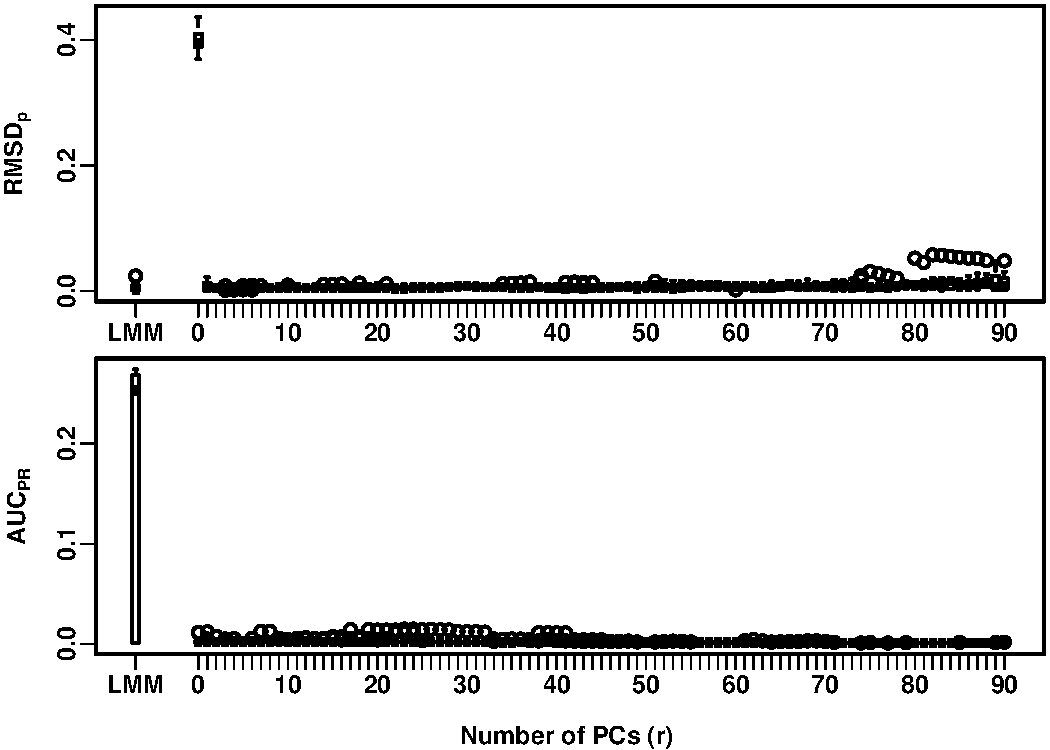
\includegraphics[width=4in]{C:/Users/yiqiy/Desktop/gas-rgls/PCA_gwas/PCA_n_1000_m_10_k_10.pdf}
  \caption{
    {\bf boxplot of rmsd and auc}
    The first panel is the boxplot of RMSD when sample size is 1000. Here the y axis represents value of rmsd and x axis is the number of PCs used in PCA.
    The second panel is the boxplot of AUC and here y axis is value of AUC. RMSD is used to measure the deviation of distribution of p values of null hypothesis from uniform distribution. In the case of multiple null hypothesis holds, the distribution of p-values of null hypothesis should approximate to unifrom distribution. The small value of RMSD implies type one error is well controlled. Regaring AUC, it's calculated by integration of predicion and recall curve. The value of AUC can be interpreted as the proportion of predictions made by this model is correct. The large AUC value implies better performance in predictive power. The result of Linear Regression is put at the position of PC equals to zero and the result of LMM is put at the position of PC equals to 91.}
  \label{fig:example}
\end{figure}

According to the first panel in Figure 1 which is the boxplot of RSMD when the number of subpopulation is 10 and sample size is 1000, it can be seen that RMSD values remain relatively high when p is smaller than 9, which satisfies the actual rank of genotype matrix or kinship matrix which is (k-1). It demonstrates that the distribution of p-values of null hypothesis deviates from the expected quantiles of uniform distribution and therefore, PCA fails to control FDR.Though the performance of PCA is relatively bad, there still exists an decreasing tendency. It indicates that when the number of PCs used in PCA is smaller than true rank of genotype matrix, PCA will benefit forom using more PCs in terms of controlling FDR. However, once the number of PCs used in PCA reaches the actual rank of genotype matrix or kinship matrix, the RSDM will junmp to a small value and in this case the value of RMSD is close to 0. It remains stable as the number of PCA increases. Apart from this, it can be seen that before the number of PCs reaches the rank of genotype matrix, the distance among minimum and maximun of RMSD is larger. It tends to be smaller after number of PCs used in PCA is larger than the rank of genotype matrix, which shows less fluctuations in terms of type 1 error controlling. The RMSD value of LM is around 0.13 and it is smaller than PCA's RMSD value when PCs used in PCA is smaller than true rank of genotype matrix. However, once the number of PCs is larger than true rank of genotype matrix, it can be seen that PCA has better performance in type one error controlling. Compared with the performance of LMM, it can be seen that both PCA and LMM controll type one error well once the number of PCs used in PCA is larger than the true rank of genotype.\\

The seond pandel of Figure 1 illustrates the pattern of AUC for the same scenario to the first panel. In this case, we can see a increasing tendency for AUC when the number of PCs is samller than the true rank of genotype or kinship matrix. Such a tendency indicates that the increase of number of PCs can increase predictive power of PCA when it is smaller than the rank of genotype matrix. Once the number of PCs used in PCA exceeds the rank of PCA, the value of AUC will be increased to around 0.8, which indicates that $80\%$ predictions of PCA are correct. After that, PCA does not benefit from adding more PCs as it can not increase the value of AUC obviously. Similarly, the range of AUC tends to be smaller than it when the number of PCs used in PCA is greater than rank of genotype matrix. It is clear that LM has better performance when  Similar to the previous pandel, PCA outperforms LM when the number of PCs is no smaller than the true rank of genotype matrix. In terms of LMM, the average AUC value is slightly higher than AUC of PCA even the number of PCs is larger than true rank of genotype matrix. \\


\subsection{PCA performance under N=100}
\begin{figure}[bp!]
  \centering
  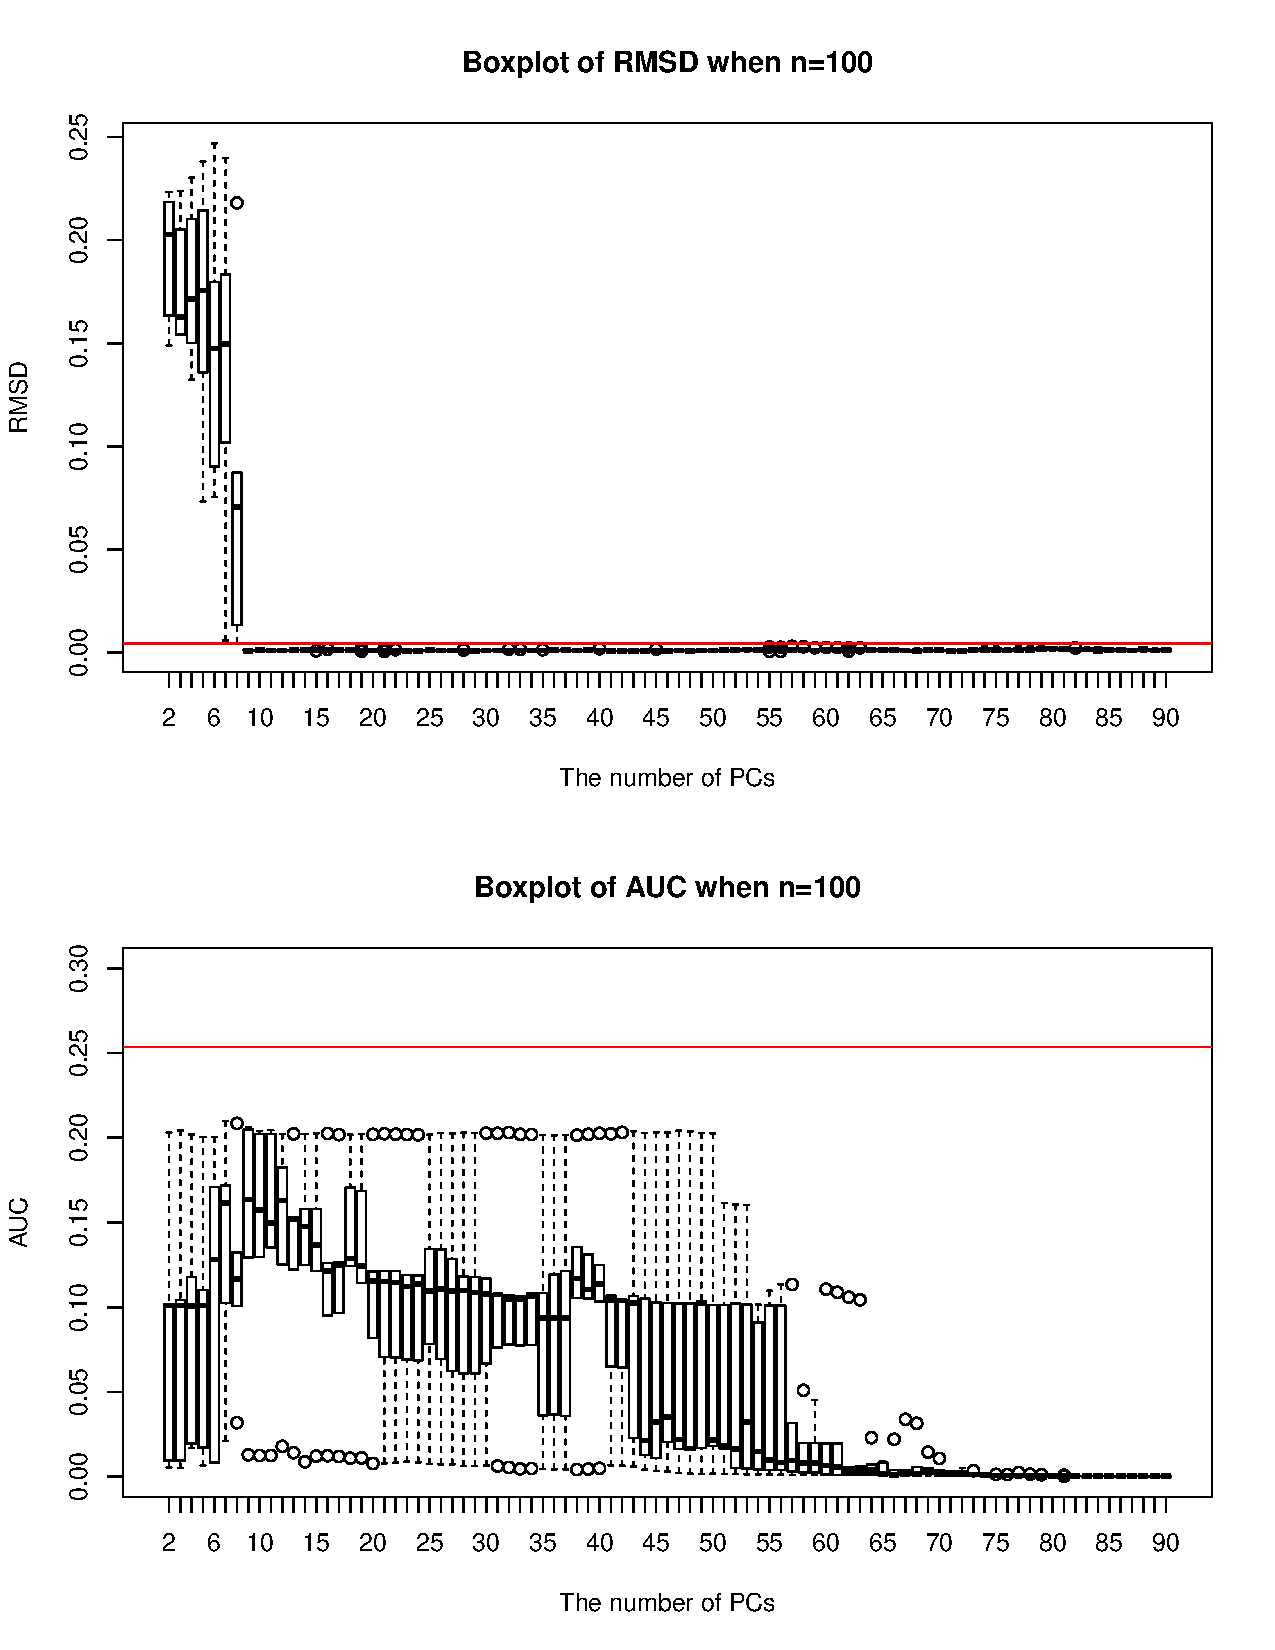
\includegraphics[width=4in]{C:/Users/yiqiy/Desktop/gas-rgls/PCA_gwas/PCA_n_100_m_10_k_10.pdf}
  \caption{
    {\bf boxplot of rmsd and auc}
    The first panel is the boxplot of RMSD when sample size is 1000. Here the y axis represents value of rmsd and x axis is the number of PCs used in PCA.
    The second panel is the boxplot of AUC and here y axis is value of AUC. RMSD is used to measure the deviation of distribution of p values of null hypothesis from uniform distribution. In the case of multiple null hypothesis holds, the distribution of p-values of null hypothesis should approximate to unifrom distribution. Therefore, we use root mean square deviation (RMSD) to measure the deviation between the distribution of p-values and uniform distribution. The small value of RMSD implies type one error is well controlled. Regaring AUC, it's calculated by integration of predicion and recall curve. The value of AUC can be interpreted as the proportion of predictions made by this model is correct. The result of Linear Regression is put at the position of PC equals to zero and the result of LMM is put at the position of PC equals to 91.}
  \label{fig:example}
\end{figure}
\subsection{PCA performance under N=100}

Then, we want to investigate the performance of PCA when samlpe size is samll. Here we set the sample size to be 100. From the first panel of Figure 2, it can be seen that the pattern is similar to the boxplot of RMSD in the case of sample size equals to 1000. It illustrates an decreasing when the number of PCs is smaller than true rank of genotype matrix. It indicates that PCA can better control type 1 error in this situation. If the number of PCs is greater than true rank of genotype matrix, the RSMD will decrease immediately and approximate to zero, which shows type one error is excellently controlled. Hence, PCA is insensitive to the smaple size in terms of RMSD or type 1 error controlling. Campored with the RMSD value of LM, RMSD value of PCA is smaller when the number of PCs is greater than 3.It implies that PCA control type one error better than LM. Moreover,the performance of LMM in this case is similar to Figure 2 which is close to previous figure. The RMSD value of LMM approximates to 0 which indicates that there is no significant difference among PCA and LMM in this csae.\\

Concerned with the boxplot of AUC, the pattern is obviously different from the boxplot of AUC when smaple size is 1000. Although we still can find an increasing pattern of AUC before the number of PCs reaches the k. However, it can be seen that there is an decreasing pattern of AUC value once the number of PCs exceeds the true rank of PCA. It demonstrates that, even though fluctuations exist, performance of PCA in terms of power can be wrose with the increase of PCs used in PCA. The position of peak of AUC in this case is located at PCs equal to 9 which is exactly the true rank of genotype. Since we take the intercept into consideration, the true rank of genotype matrix equals to the number of subpopulation minus one. The bell-shaled distribution of AUC boxpolot implies that PCA receives punishment in power once the number of PCs used in PCA is larger than true rank of genotype matrix. Moreover, in terms of LM, it can be seen that even only one PC is used in PCA, the AUC value of PCA is still no worse than LM. However, when  excessive PCs are used, performance of LMM can be better with a larger AUC value. Considering LMM, the average` AUC value is 0.25, whereas, the maximum AUC of PCA is 0.2 and it decreases immediately due to the excessive use of PCs. In this case, LMM performs better than PCA in terms of power. \\




\begin{figure}[bp!]
  \centering
  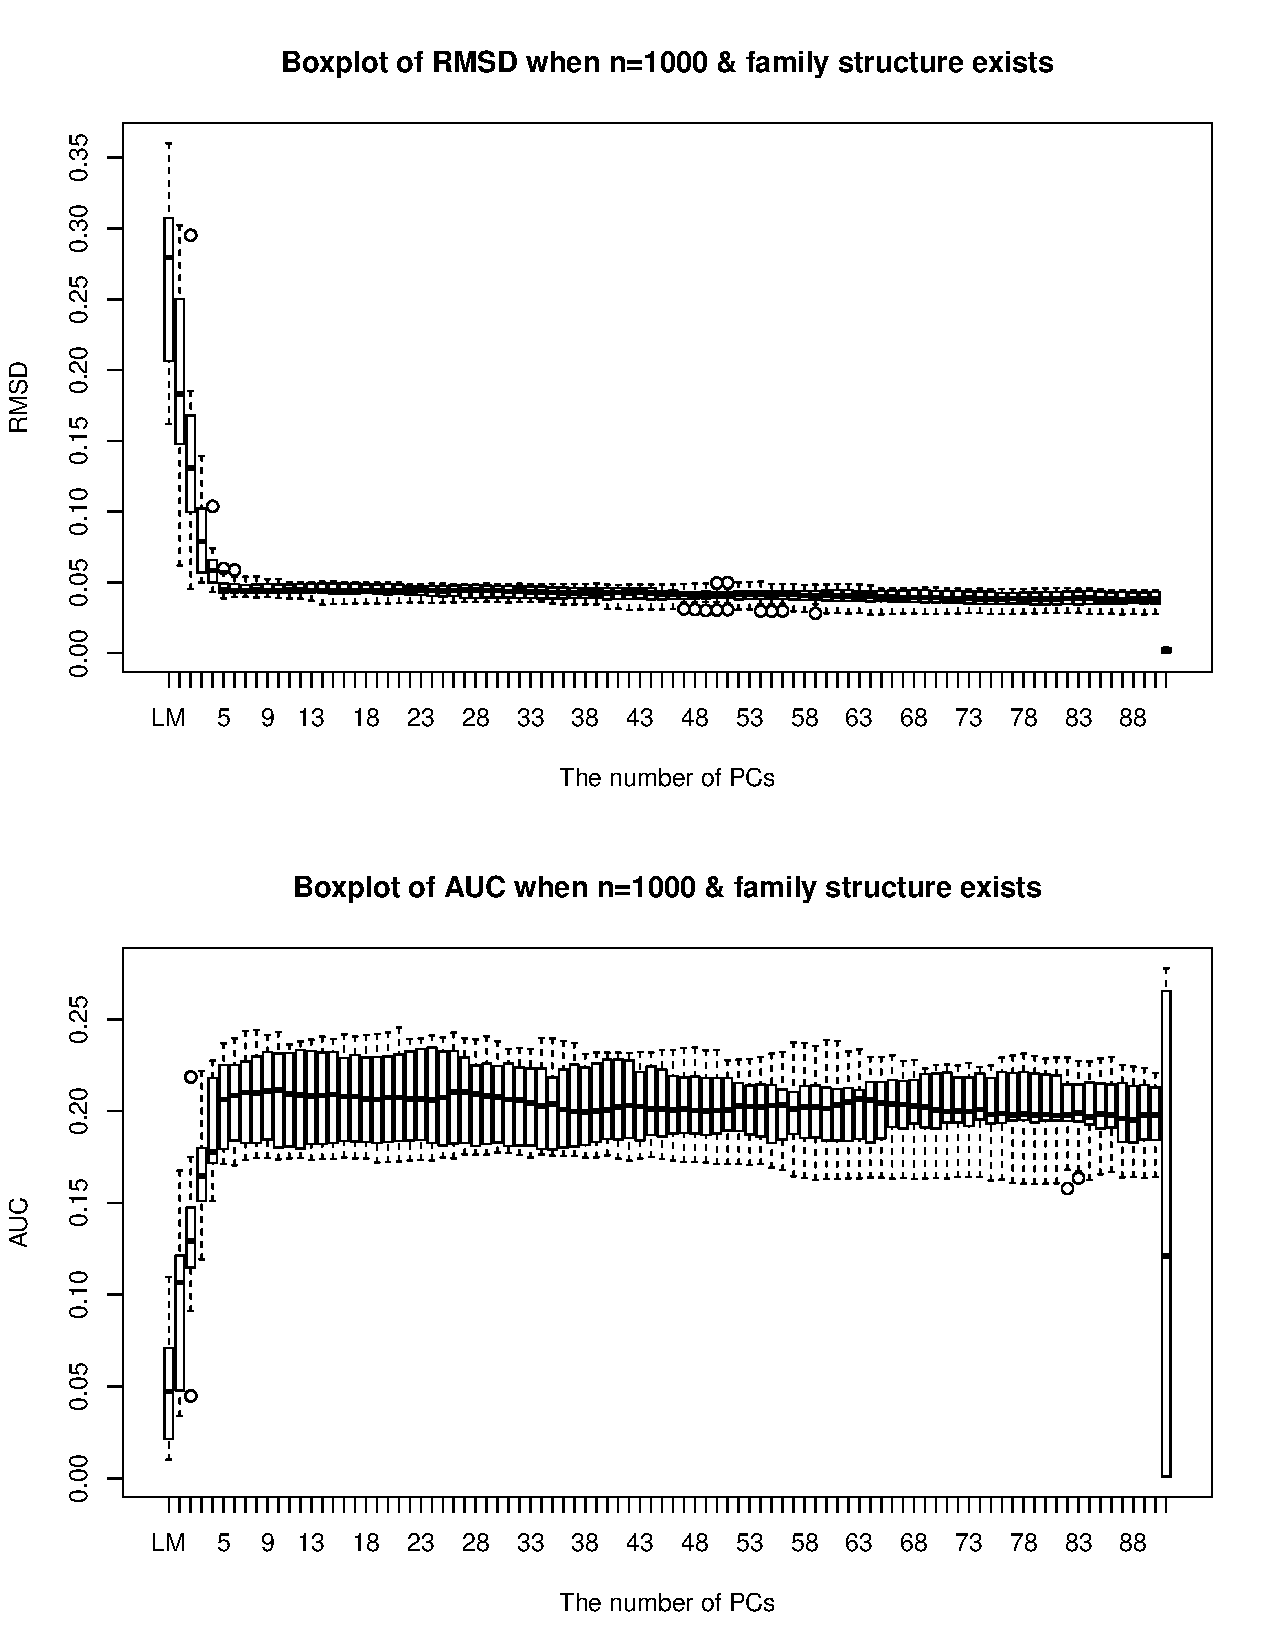
\includegraphics[width=4in]{C:/Users/yiqiy/Desktop/gas-rgls/PCA_gwas/PCA_n_1000_m_100_family_structure.pdf}
  \caption{
    {\bf boxplot of rmsd and auc}
    The first panel is the boxplot of RMSD when sample size is 100.}
  \label{fig:example}
\end{figure}

\subsubsection{PCA performance when familty structure exists}

The introduction of family structure will make the original admixture populatio more complicated. In this csae, we assume that there are 20 generations in total while other factors fixed. Based on the result of the first panel in figure 3 indicates that there is a decreasing pattern of RMSD for the first three PCs. It addition, the value of RMSD in this situation is large, which indicates that the distribution of p-value of null hypothesis does not approximate to uniform distribution. It illustrates that PCA fails to control type one error when the number of PCs is not enough. When the number of PCs is larger than 4, values of RMSD beome stable around 0.05 which demonstrates that there exists evidence of the distribution of p-value of null hypothesis does not deviate from uniform distribution but the evidence is weaker than previous simulation where RSDM approximates to 0. Considering the range of RMSD, it decreases first and then begins to increase. It shows that excessive use of PCs will lead to extra variance.For AUC, it illustrates an increasing tendency for the first three PCs. When the number of PCs is larger than 3, AUC fluctuates around 0.2. This shows the power of PCA is small and hence, PCA's performance is not pretty well in this csae in terms of power even though enough PCs are used. 


\section{Discussion}
\subsection{PCA GWAS fails without enough PCs}
Right now, both LMM and PCA have become standard approaches to correct for admixture population. In current PCA GWAS research, the number of PCs used in PCA is ususally assmued to be 10. For instance, based on the simulation of Hoffman (2013), 10 PCs are randomly selected from the first 30 PCs. Furthermore, Genevieve et al. (2019) also performed PCA GWAS for 26 traits with first 10 PCs. According to the result of Genevieve et al. (2019), the correlation plot between SNP genotype and PC1–PC10 illustrates different populations has different correlations over some PCs. It seems that there exists a tradition that when PCA GWAS is performed, the top 10 PCs will be used. Since the result of PCA GWAS in this convention is good, right now most paprs will assume the number of PCs used in PCA GWAS to be 10. However, in this paper, we further investigate about the optimal choice of number of PCA under different population structures. In most current research, the number of subpopulation is smaller 10 and thus, based on results of previous three scenarios, the number of PCs used in PCA is enough which certifies the good performance of PCA  in current research. For instance, based on the scatter plot of first two principal components with HapMap3 dataset which contains 11 populations, it can be divided into three subpopulations (Gad and Machiel, 2014). On the contraty, the lack of PCs will lead to the failure of PCA regardless of the sample size or family structure in both type one error and power. 


\subsection{PCA GWAS still works even too many PCs are used}
PCA GWAS is still robust even though PCs are excessively used for type one error controlling. However, for power, it will receive punishment if the number of PCs are excessive and the sample size is small. Jason and Anna (2009) point out that PCA with large sample size has better sample size than it with small sample size. This is because that PCA with large sample size can have smaller probability error and larger accuracy of population estimation ( Jason and Anna ,2009). The small sample size in our research project only has 100 individuals in total. In a GWAS study, this is an extreme situation which it not realistic in research. The AUC boxplot of small sample size indicates that the peak of AUC is close to AUC value for large sample size. This may result from that the number of causal loci in small sample size is reduced from 100 to 10.However, the boxplot of AUC has a bell shap with downward-sloping line on each side of the peak. It demonstrates that in small sample size, punishment of excessive use of PCs will come occur immdeiately. Previous simulations of PCA has not taken into cosideration. 

\subsection{PCA GWAS fails with the existence are close relatives }

\subsection{LMM outperforms PCA }
Wang et al. (2013) argues that mixed effects model is preferred in the case of existence cryptic relatedness but not population stratification. However, based on the result of our simulations, it can be seen that in both large sample size and small sample size, LMM are slightly better than PCA in terms of power. When sample size is large such as the scenario in figure 1 panel B, it can be seen that although both two methods's are not good. However, the maximum AUC value of PCA is around 0.25 and LMM's AUC value is slightly larger than PCA. In addition to this, in the case of small smaple size, advantage of LMM is more obvious. As mentioned before, PCA will receive punishment when the number of PCs is much larger than the true rank of genotype matrix. The maximum of AUC value of PCA in this scenario decreases to 0.2 and the average AUC value of LMM is around 0.24. This two simulations illustrates that 

\end{document}
